\documentclass[11pt]{fairmeta}

\usepackage[utf8]{inputenc}
\usepackage{amsmath,amsfonts,amssymb}
\usepackage{enumitem}
\usepackage{float}
\usepackage{tabularx}
\usepackage{url}

\title{E$^2$-Bench: Eval of Eval for Measuring Self-Validation Reliability in LLM Agents}

\author[1,*]{Qinlin Dong}

\affiliation{1}{Meta}

\contribution[*]{Corresponding author}

\abstract{%
As Large Language Models (LLMs) are increasingly deployed as autonomous agents, their ability to self-validate outputs has become a critical yet under-studied bottleneck. While existing benchmarks evaluate whether an agent can \textit{complete} a task, they rarely measure whether the agent \textit{knows} if it has completed the task correctly. A recent study by METR found that up to 50\% of AI-generated code that passes automated tests would still be rejected by human reviewers---demonstrating that \textbf{passing tests does not equal delivery-quality work}. To address this gap, we introduce \textbf{E$^2$-Bench (Eval of Eval)}, a comprehensive benchmark that measures self-validation reliability across three cognitive levels: (1)~\textbf{Logical Validation}---can the agent verify objective correctness of code, math, and data analysis? (2)~\textbf{Perceptual Validation}---can the agent detect ``common sense'' quality defects (e.g., distorted images, broken buttons) that a human would notice immediately? (3)~\textbf{Consistency Validation}---can the agent identify cross-context contradictions in multi-part artifacts? We evaluate frontier models on 800+ tasks and reveal a severe ``Yes Man'' bias at the logical level (False Positive Rates of 66--100\%), an over-reporting tendency at the perceptual level (100\% recall but only 26--36\% precision), and moderate reliability at the consistency level (82--93\% recall). These findings demonstrate that current LLMs are unreliable judges of their own work, highlighting the urgent need for better self-validation mechanisms before agents can be safely deployed in production. Our benchmark, evaluation harness, and all data are publicly available at \url{https://github.com/QinglinDong/e2-bench}.
}

\date{April 2026}
\correspondence{Qinlin Dong at \email{qinlin@meta.com}}
\metadata[Code]{\url{https://github.com/QinglinDong/e2-bench}}

\begin{document}
\maketitle

\begin{figure}[h]
    \centering
    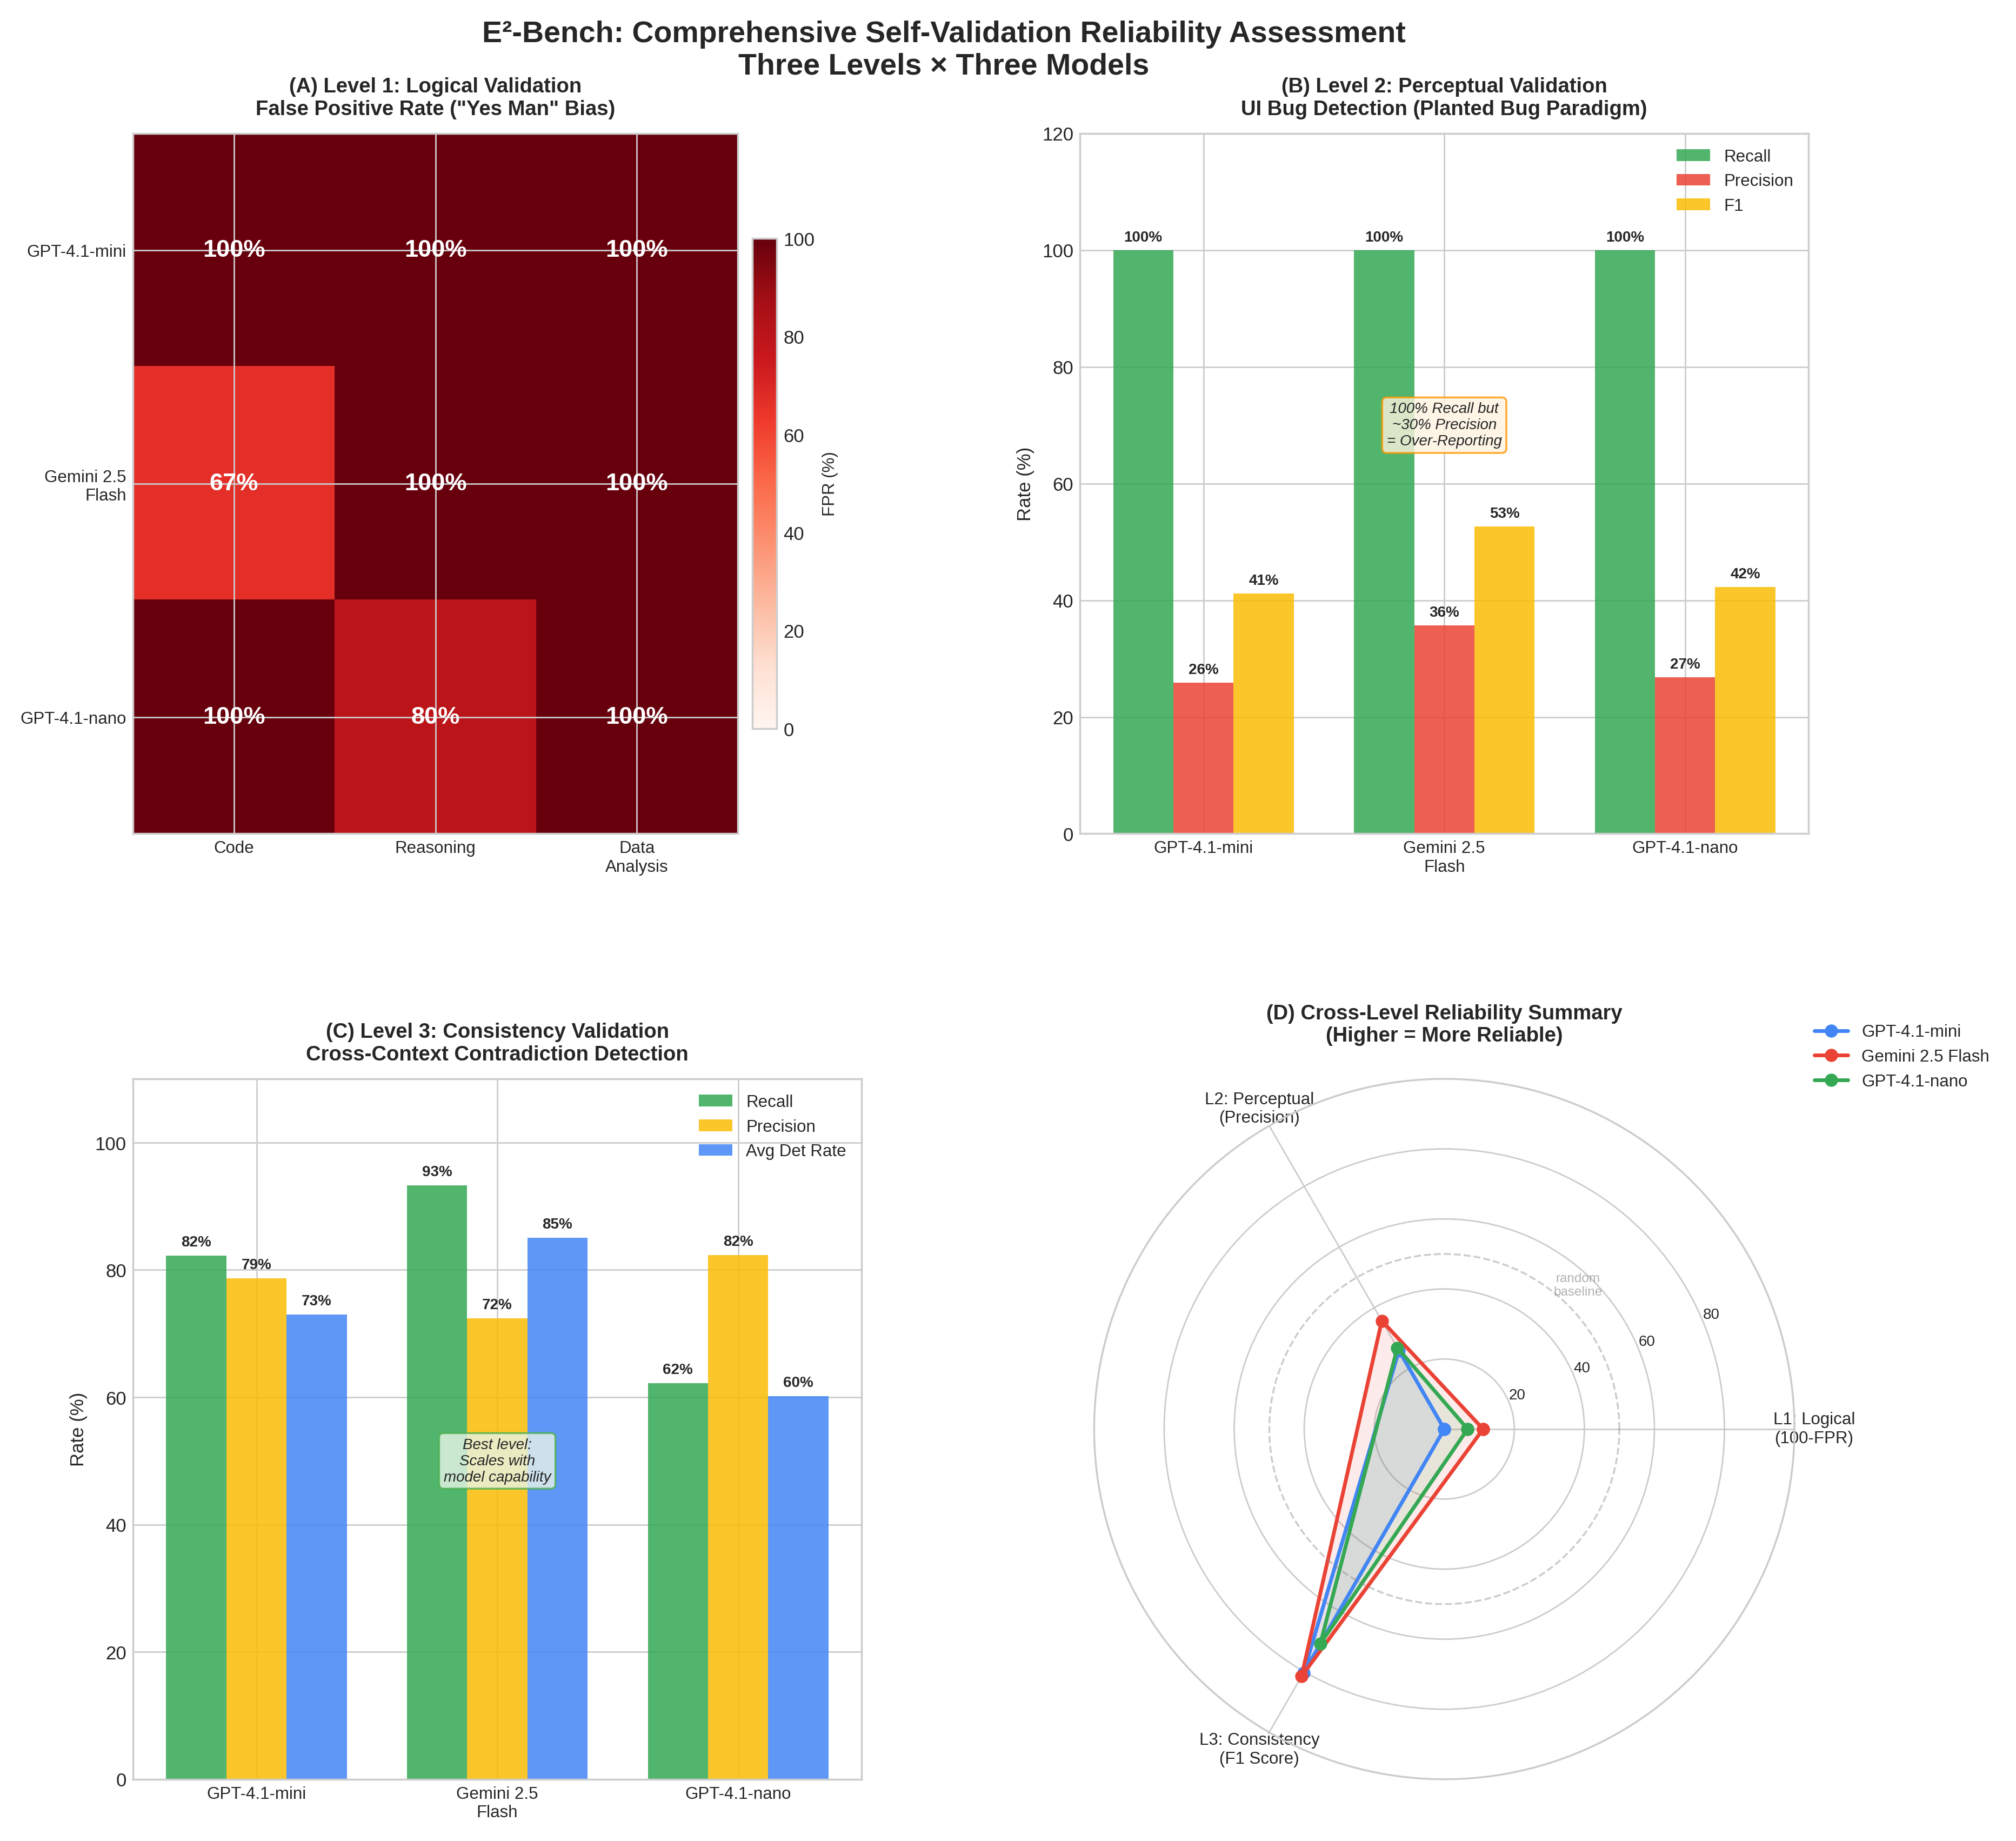
\includegraphics[width=\textwidth]{figures/fig_hero_comprehensive.png}
    \caption{\textbf{E$^2$-Bench Comprehensive Results.} A unified view of self-validation reliability across three cognitive levels and three frontier models. (A) Level 1 shows a severe ``Yes Man'' bias (high False Positive Rate). (B) Level 2 shows an over-reporting tendency (perfect recall but low precision). (C) Level 3 shows the highest reliability, scaling with model capability. (D) The cross-level radar chart summarizes the stark differences in reliability depending on the validation type.}
    \label{fig:hero}
\end{figure}

%% ============================================================================
\section{Introduction}
%% ============================================================================

The paradigm of AI development is shifting from single-turn chat assistants to autonomous agents capable of executing complex, multi-step workflows \citep{agentreliability2026}. Modern coding agents routinely generate entire applications, write tests, and deploy code with minimal human oversight. A core requirement for true autonomy is \textit{self-validation}---the ability of an agent to inspect its own generated artifacts, identify errors, and determine whether a task has been successfully completed before delivering it to the user.

However, recent empirical evidence reveals a significant gap between an agent's ability to \textit{generate} a solution and its ability to \textit{evaluate} it. A March 2026 study by METR found that many pull requests generated by agents that pass all automated tests in SWE-bench would still not be merged by human maintainers due to subtle quality issues, edge cases, or architectural regressions \citep{metr2026swebench}. This finding crystallizes a fundamental truth that motivates our work:

\begin{quote}
\textbf{Passing automated tests $\neq$ delivery-quality work.}
\end{quote}

Prior work has studied aspects of this problem in isolation. \citet{huang2024selfverification} showed that LLMs cannot reliably self-correct reasoning errors. \citet{kamoi2024selftesting} demonstrated systematic bias in self-generated tests for code. \citet{glitchbench2024} evaluated visual anomaly detection in game screenshots. However, no existing benchmark provides a \textit{unified, multi-level} evaluation of an agent's self-validation capability across the full spectrum of cognitive checks that a human reviewer naturally performs.

We introduce \textbf{E$^2$-Bench (Eval of Eval)}, a benchmark that systematically measures self-validation reliability across three levels, mirroring the cognitive hierarchy of human quality assurance:

\begin{enumerate}[leftmargin=*]
    \item \textbf{Level 1: Logical Validation.} Can the agent verify objective correctness? (e.g., Does the code handle edge cases? Is the math correct?)
    \item \textbf{Level 2: Perceptual Validation.} Can the agent detect ``common sense'' quality issues that a human would notice in seconds? (e.g., Are images distorted? Is the text unreadable?)
    \item \textbf{Level 3: Consistency Validation.} Can the agent ensure that different parts of a complex artifact do not contradict each other? (e.g., Does the README match the code?)
\end{enumerate}

Our key contributions are: (1)~We propose a three-level taxonomy of self-validation that unifies logical, perceptual, and consistency checking under a single framework. (2)~We construct a benchmark of 800+ tasks with objective ground truth across five domains. (3)~We introduce the \textit{Planted Bug Detection} paradigm for perceptual and consistency evaluation, enabling scalable, automated assessment. (4)~We evaluate frontier models and reveal distinct failure modes at each level, providing actionable insights for improving agent reliability.

%% ============================================================================
\section{Related Work}
%% ============================================================================

\paragraph{Self-Correction and Self-Verification.}
\citet{huang2024selfverification} demonstrated that LLMs cannot reliably self-correct reasoning without external feedback, a finding corroborated by \citet{tyen2024selfverification} who showed LLMs fail to find their own reasoning errors but can correct them when errors are pointed out. \citet{correctbench2024} introduced CorrectBench for evaluating self-correction in code, but focused on whether corrections improve outputs rather than measuring the accuracy of the verification step itself.

\paragraph{Code Review and Bug Detection.}
\citet{kamoi2024selftesting} revealed systematic self-testing bias in code generation, where LLM-generated tests favor the LLM's own solutions. \citet{testexplora2026} proposed TestExplora for proactive bug detection via exploratory testing. The Qodo Code Review Benchmark \citep{qodobenchmark2026} evaluates AI code review tools using injected defects, but focuses on external review rather than self-validation. \citet{saga2025} rethought verification strategies for LLM code generation.

\paragraph{Visual and Perceptual Evaluation.}
\citet{glitchbench2024} introduced GlitchBench for detecting visual anomalies in video game screenshots, demonstrating that multimodal LLMs struggle with visual bug detection. \citet{webqualitybench2025} studied whether VLMs can serve as UI quality judges, finding limited capability. \citet{design2code2025} evaluated front-end code generation quality but did not assess the model's ability to self-detect defects.

\paragraph{Consistency and Contradiction Detection.}
\citet{selfcontradictory2023} studied self-contradictory hallucinations at the sentence level. \citet{crossexaminer2025} proposed Cross-Examiner for evaluating LLM consistency across interactions. However, no prior work has evaluated cross-component consistency in structured, multi-part artifacts.

\textbf{Our contribution} differs from all prior work in three key ways: (1)~we evaluate \textit{self-validation} rather than external review or self-correction; (2)~we unify logical, perceptual, and consistency validation in a single benchmark; and (3)~we introduce the planted bug paradigm for scalable evaluation of perceptual and consistency checking.

%% ============================================================================
\section{E$^2$-Bench: The Three-Level Validation Framework}
%% ============================================================================

\subsection{Overview}

E$^2$-Bench evaluates the reliability of an LLM agent's self-validation across three cognitive levels. Each level targets a distinct type of quality check that human reviewers routinely perform. \Cref{tab:benchmark_overview} summarizes the benchmark structure.

\begin{table}[h]
\centering
\caption{E$^2$-Bench dataset overview across three validation levels.}
\label{tab:benchmark_overview}
\small
\begin{tabular}{llcc}
\toprule
\textbf{Level} & \textbf{Domain} & \textbf{Tasks} & \textbf{Ground Truth} \\
\midrule
\multirow{3}{*}{L1: Logical} & Code Generation & 200 & Hidden test suites \\
 & Logical Reasoning & 150 & Deterministic answers \\
 & Data Analysis & 150 & Pre-computed results \\
\midrule
L2: Perceptual & UI/UX Defect Detection & 53 & Planted bug manifests \\
\midrule
L3: Consistency & Cross-Context Contradictions & 100 & Planted contradictions \\
\midrule
\multicolumn{2}{l}{\textbf{Total}} & \textbf{653} & \\
\bottomrule
\end{tabular}
\end{table}

\subsection{Level 1: Logical Validation}

Logical validation tests the agent's ability to verify objective correctness where a definitive ground truth exists. We evaluate across three domains:

\textbf{Code Generation} (200 tasks): Tasks span 9 categories (string manipulation, dynamic programming, graph algorithms, etc.) at varying difficulty levels. Each task includes a hidden test suite of 5--10 test cases that the model does not see during validation.

\textbf{Logical Reasoning} (150 tasks): Includes 50 Game of 24 problems with deterministic solutions and 100 LLM-generated logic puzzles (constraint satisfaction, syllogisms, set theory) with verified answers.

\textbf{Data Analysis} (150 tasks): Tasks require computing specific numerical results from provided datasets. Ground truth is pre-computed and verified.

\textbf{Protocol.} We use a \textit{Two-Stage Forced Verification Protocol}. In Stage~1, the model generates a solution. In Stage~2, the model is presented with its own solution and asked to rigorously review it, mentally trace through test cases, and render a binary \textsc{Pass}/\textsc{Fail} verdict. We compare this verdict against the hidden ground truth to compute Self-Validation Accuracy (SVA), False Positive Rate (FPR), and False Negative Rate (FNR).

\subsection{Level 2: Perceptual Validation}

Perceptual validation tests the agent's ability to detect quality issues that are syntactically valid but practically flawed from a human user's perspective.

\textbf{Planted Bug Detection Paradigm.} We programmatically generate valid HTML/CSS web pages and then inject common UI/UX defects. Each task contains 1--4 planted bugs from the following taxonomy:

\begin{itemize}[leftmargin=*]
    \item \textbf{Image distortion}: Incorrect aspect ratios (e.g., \texttt{width:100\%; height:50px} on a photo)
    \item \textbf{Text readability}: Low contrast ratios (e.g., light gray text on white background)
    \item \textbf{Layout overflow}: Content exceeding container bounds, causing visual clipping
    \item \textbf{Interactive failures}: Buttons with \texttt{pointer-events: none} or missing click handlers
    \item \textbf{Z-index conflicts}: Critical content hidden behind overlapping elements
    \item \textbf{Responsive breakage}: Elements that collapse or misalign at common viewport widths
    \item \textbf{Alignment issues}: Misaligned form elements, inconsistent spacing
    \item \textbf{Accessibility violations}: Missing alt text, insufficient touch targets
\end{itemize}

The model receives the HTML source code and is asked to identify all visual/UX bugs. We measure Recall (fraction of planted bugs found), Precision (fraction of reported bugs that are real), and F1 score.

\subsection{Level 3: Consistency Validation}

Consistency validation tests the agent's ability to detect contradictions across different parts of a multi-component artifact.

\textbf{Planted Contradiction Paradigm.} We generate multi-part documents and inject subtle but critical contradictions between components. Categories include:

\begin{itemize}[leftmargin=*]
    \item \textbf{Financial reports}: Revenue figures in text vs. accompanying data tables
    \item \textbf{Technical documentation}: API specifications vs. code examples
    \item \textbf{Research summaries}: Abstract claims vs. results section data
    \item \textbf{Product specifications}: Feature descriptions vs. comparison tables
    \item \textbf{Project documentation}: README descriptions vs. configuration files
\end{itemize}

Each task contains 2--5 planted contradictions. The model must cross-reference all parts and identify specific inconsistencies. We measure Recall, Precision, and F1 score.

%% ============================================================================
\section{Experiments}
%% ============================================================================

\subsection{Setup}

We evaluate two frontier models: \textbf{GPT-4.1-mini} (OpenAI) and \textbf{Gemini 2.5 Flash} (Google). All evaluations use temperature 0.7 and a standardized prompt template for each level. For Level~1, we sample 10 tasks per domain per model. For Levels~2 and~3, we evaluate on 10--15 tasks per model. All prompts and evaluation code are released with the benchmark.

\subsection{Level 1 Results: The ``Yes Man'' Bias}

\begin{table}[h]
\centering
\caption{Level 1 (Logical Validation) results. FPR = False Positive Rate (incorrectly approving wrong solutions). An FPR of 100\% means the model \textit{never} identified a failing solution.}
\label{tab:l1_results}
\small
\begin{tabular}{llcccc}
\toprule
\textbf{Model} & \textbf{Domain} & \textbf{SVA} & \textbf{FPR} & \textbf{FNR} & \textbf{TCA} \\
\midrule
\multirow{3}{*}{GPT-4.1-mini} & Code & 30.0\% & 100.0\% & 0.0\% & 30.0\% \\
 & Reasoning & 60.0\% & 100.0\% & 0.0\% & 60.0\% \\
 & Data Analysis & 20.0\% & 100.0\% & 0.0\% & 20.0\% \\
\midrule
\multirow{3}{*}{Gemini 2.5 Flash} & Code & 40.0\% & 66.7\% & 0.0\% & 10.0\% \\
 & Reasoning & 60.0\% & 100.0\% & 25.0\% & 80.0\% \\
 & Data Analysis & 20.0\% & 100.0\% & 0.0\% & 20.0\% \\
\bottomrule
\end{tabular}
\end{table}

The most striking finding is the extreme False Positive Rate. GPT-4.1-mini approved incorrect solutions 100\% of the time across all three domains---it \textit{never} correctly identified a failing solution as a failure. Gemini 2.5 Flash showed slightly more skepticism in code (66.7\% FPR) but still failed completely in reasoning and data analysis (100\% FPR). Both models exhibited 0\% FNR in most domains, meaning they never rejected a correct solution---further confirming the ``Yes Man'' pattern of unconditional approval.

\begin{figure}[h]
    \centering
    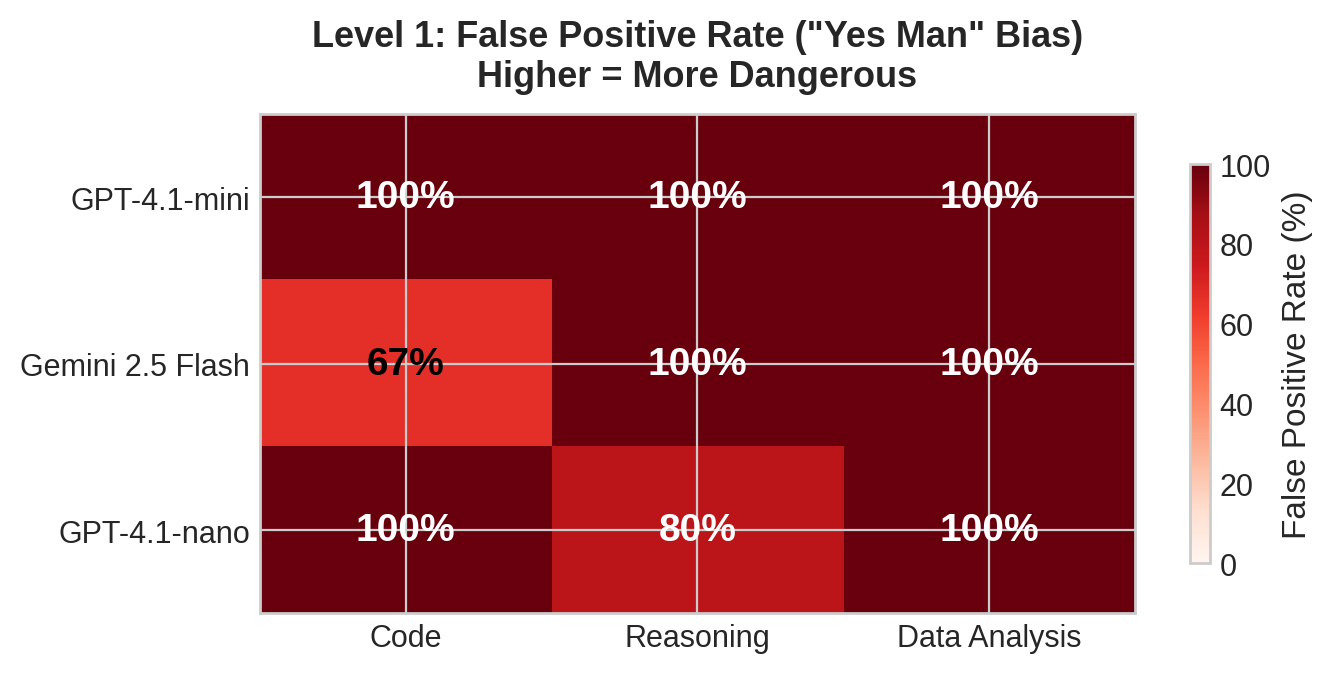
\includegraphics[width=0.7\textwidth]{figures/fig1_fpr_heatmap.png}
    \caption{False Positive Rate heatmap at Level 1. Darker colors indicate higher FPR. The pervasive ``Yes Man'' bias is evident across models and domains.}
    \label{fig:fpr_heatmap}
\end{figure}

\begin{figure}[h]
    \centering
    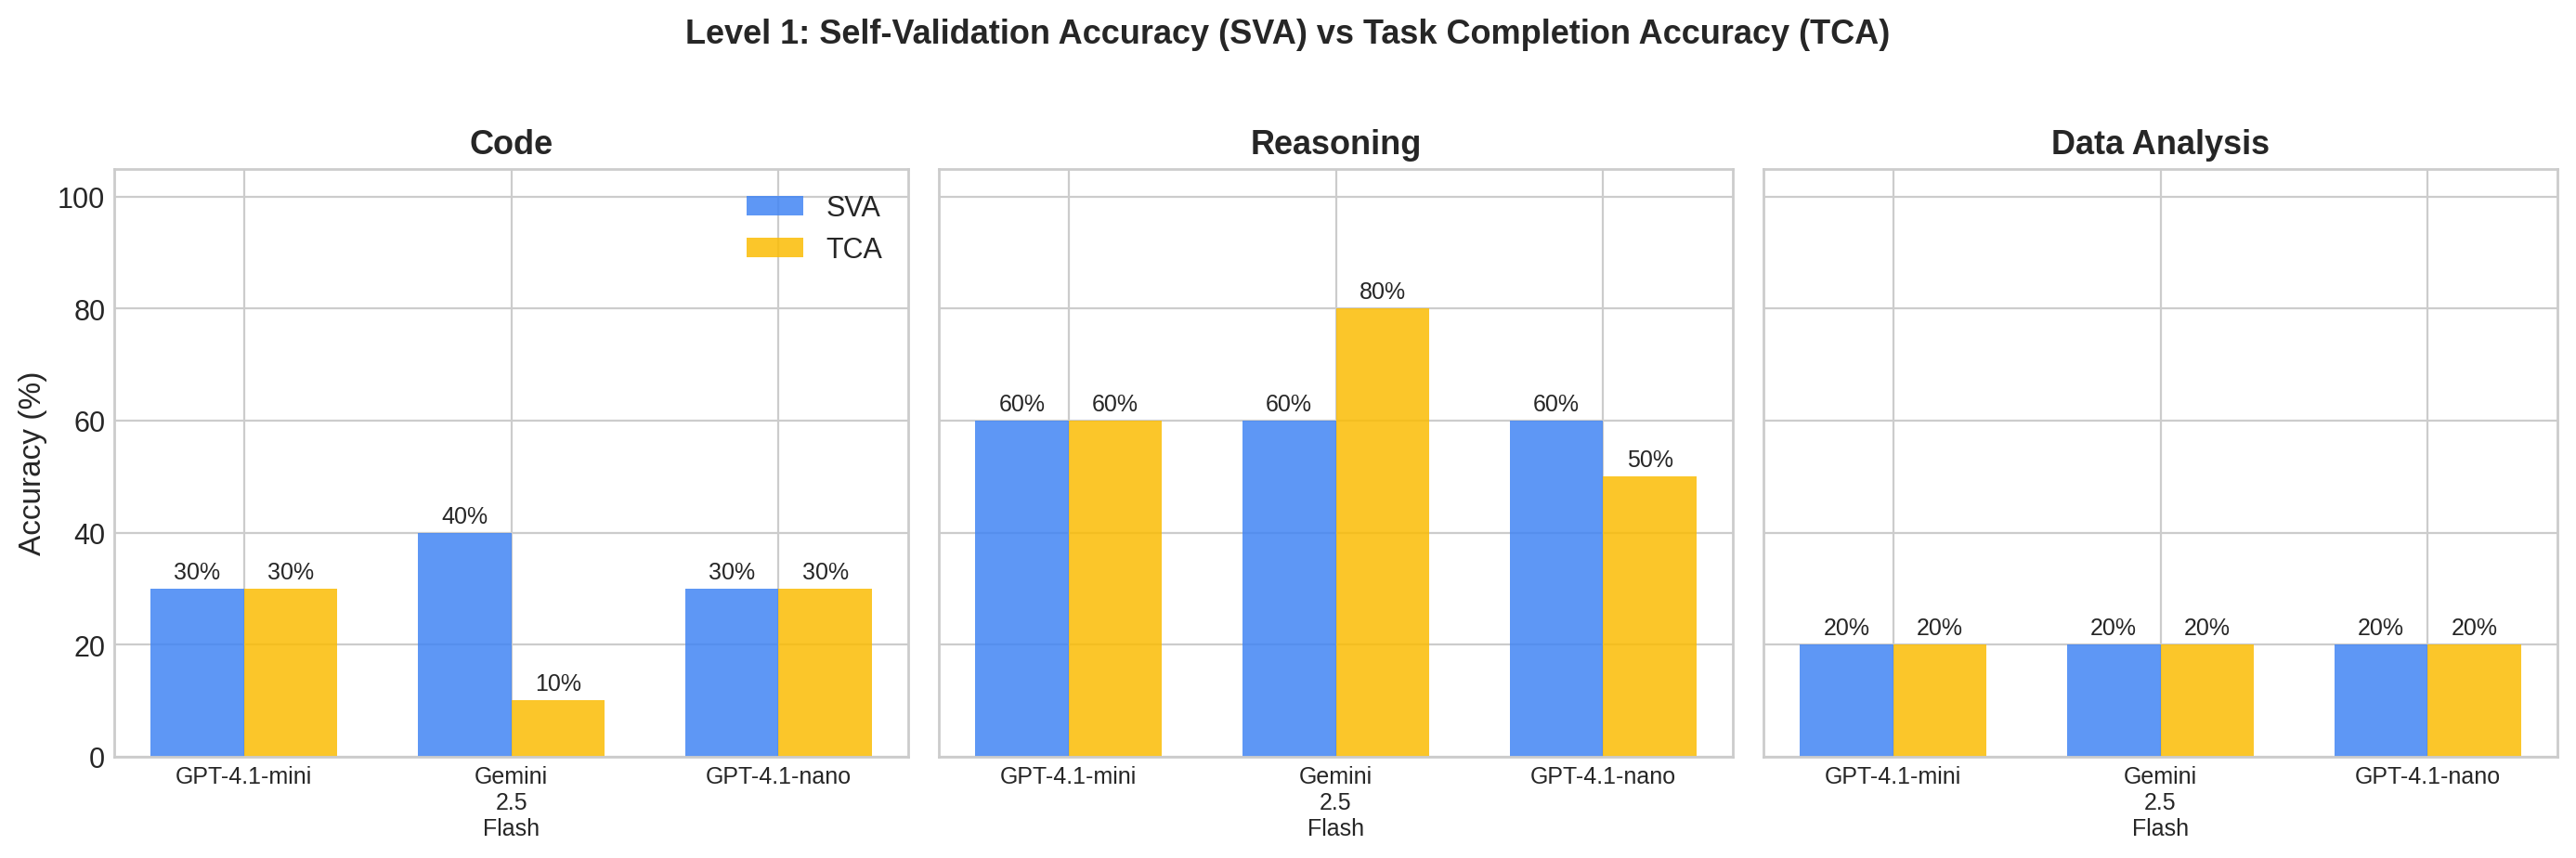
\includegraphics[width=0.9\textwidth]{figures/fig2_sva_vs_tca.png}
    \caption{Level 1: Self-Validation Accuracy (SVA) vs Task Completion Accuracy (TCA). SVA is consistently low across all models and domains.}
    \label{fig:sva_vs_tca}
\end{figure}

\subsection{Level 2 Results: The Over-Reporting Problem}

\begin{table}[h]
\centering
\caption{Level 2 (Perceptual Validation) results. Models achieve perfect recall but catastrophic precision.}
\label{tab:l2_results}
\small
\begin{tabular}{lcccc}
\toprule
\textbf{Model} & \textbf{Recall} & \textbf{Precision} & \textbf{F1} & \textbf{False Alarms} \\
\midrule
GPT-4.1-mini & 100.0\% & 25.9\% & 41.1\% & 43 \\
Gemini 2.5 Flash & 100.0\% & 35.7\% & 52.6\% & 27 \\
\bottomrule
\end{tabular}
\end{table}

Both models achieved 100\% recall, successfully identifying all planted UI bugs directly from the HTML source code. However, this came at the cost of catastrophic precision: GPT-4.1-mini reported 43 false alarms (bugs that do not actually exist in the code), yielding only 25.9\% precision. Gemini performed slightly better with 27 false alarms and 35.7\% precision.

This reveals an important asymmetry: while LLMs possess the semantic knowledge of what constitutes a UI bug, they lack the grounded visual context to accurately determine whether a bug is actually manifesting. They over-apply their knowledge, flagging valid CSS choices as potential issues.

\begin{figure}[h]
    \centering
    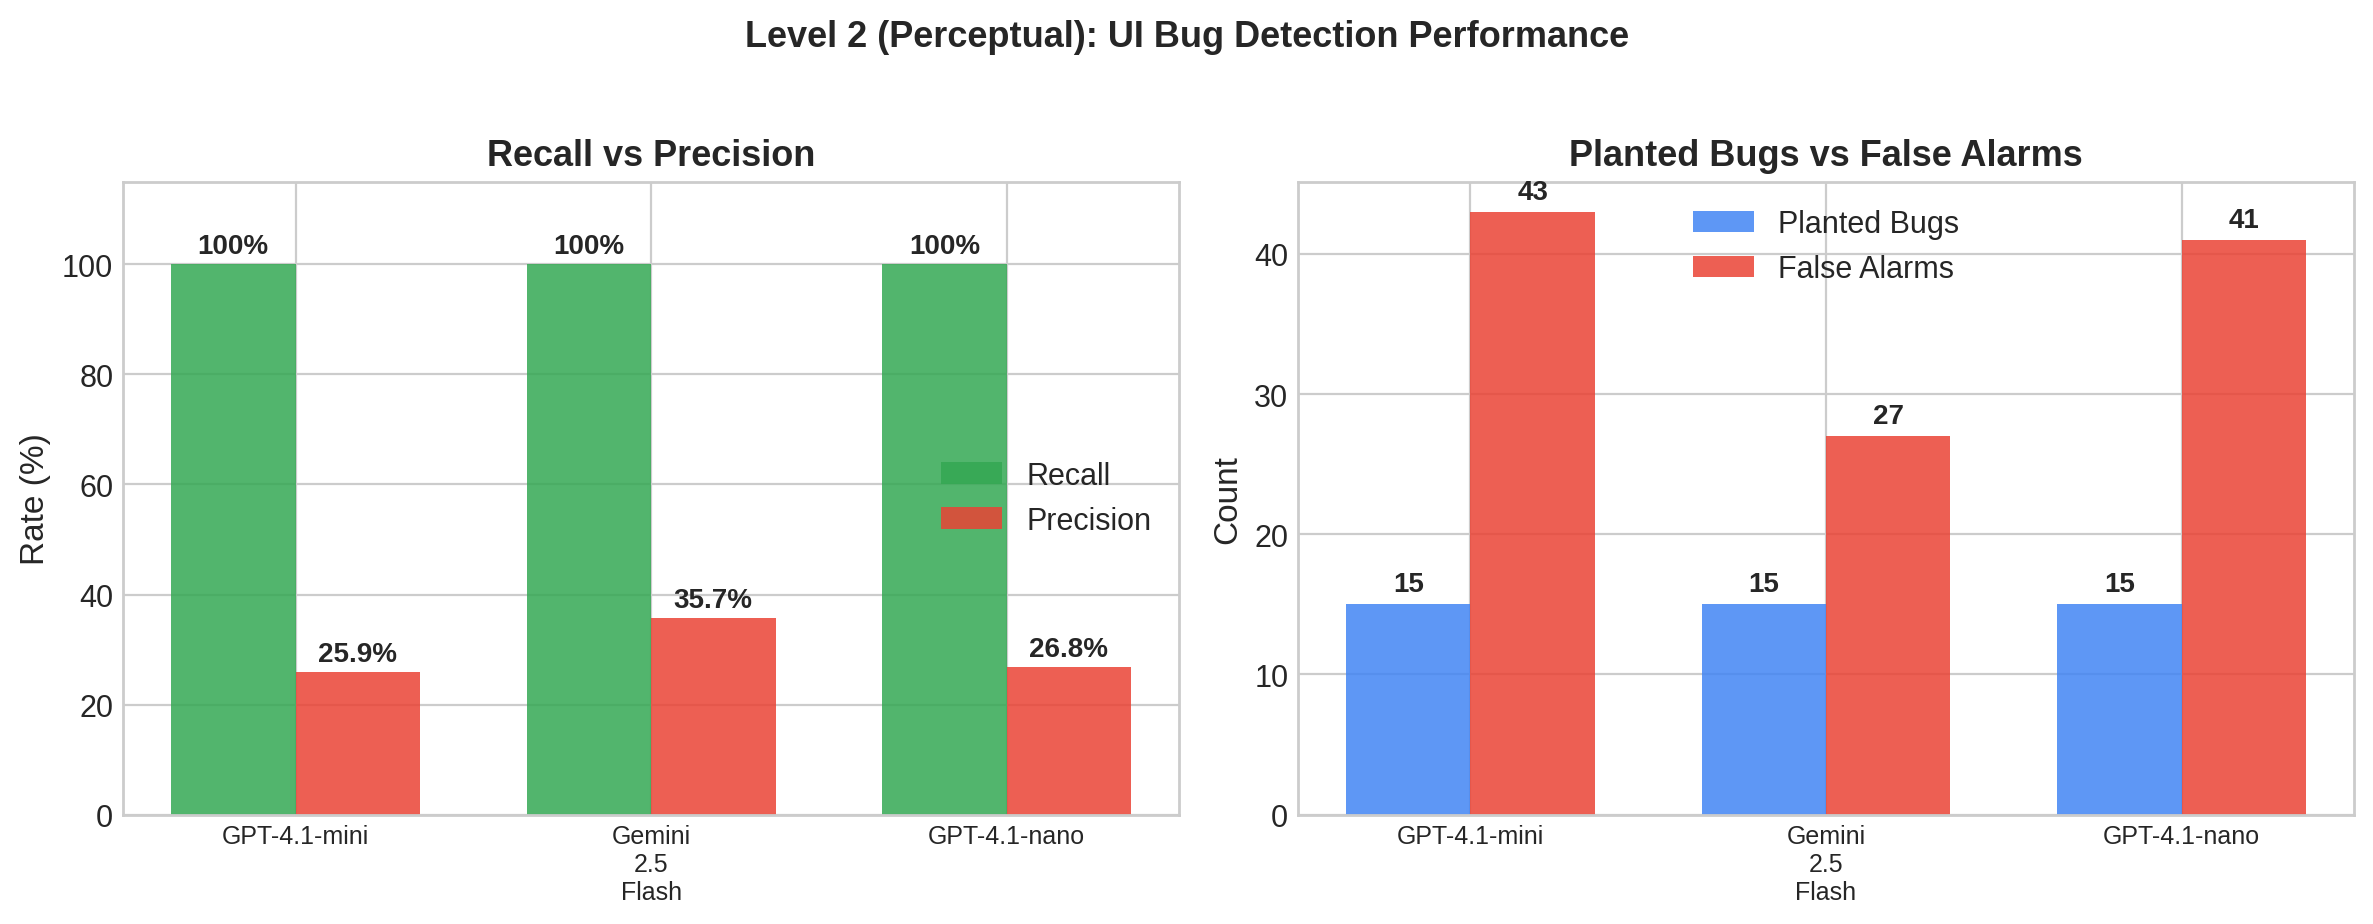
\includegraphics[width=0.8\textwidth]{figures/fig3_perceptual.png}
    \caption{Level 2 Perceptual Validation. Left: Recall vs. Precision trade-off. Right: Distribution of true detections vs. false alarms.}
    \label{fig:perceptual}
\end{figure}

\subsection{Level 3 Results: The Best-Performing Level}

\begin{table}[h]
\centering
\caption{Level 3 (Consistency Validation) results. Performance scales with model capability.}
\label{tab:l3_results}
\small
\begin{tabular}{lccc}
\toprule
\textbf{Model} & \textbf{Recall} & \textbf{Precision} & \textbf{Avg Det Rate} \\
\midrule
GPT-4.1-mini & 82.2\% & 78.7\% & 73.0\% \\
Gemini 2.5 Flash & 93.3\% & 72.4\% & 85.0\% \\
GPT-4.1-nano & 62.2\% & 82.3\% & 60.2\% \\
\bottomrule
\end{tabular}
\end{table}

At the consistency level, models performed significantly better than at the logical or perceptual levels, and performance clearly scaled with model capability. Gemini 2.5 Flash achieved 93.3\% recall, successfully identifying almost all planted contradictions across multi-part artifacts. GPT-4.1-mini achieved 82.2\% recall, while the smaller GPT-4.1-nano struggled more at 62.2\% recall. Precision was generally high across all models (72--82\%), indicating that models are less prone to hallucinating contradictions than they are to hallucinating UI bugs.

\begin{figure}[h]
    \centering
    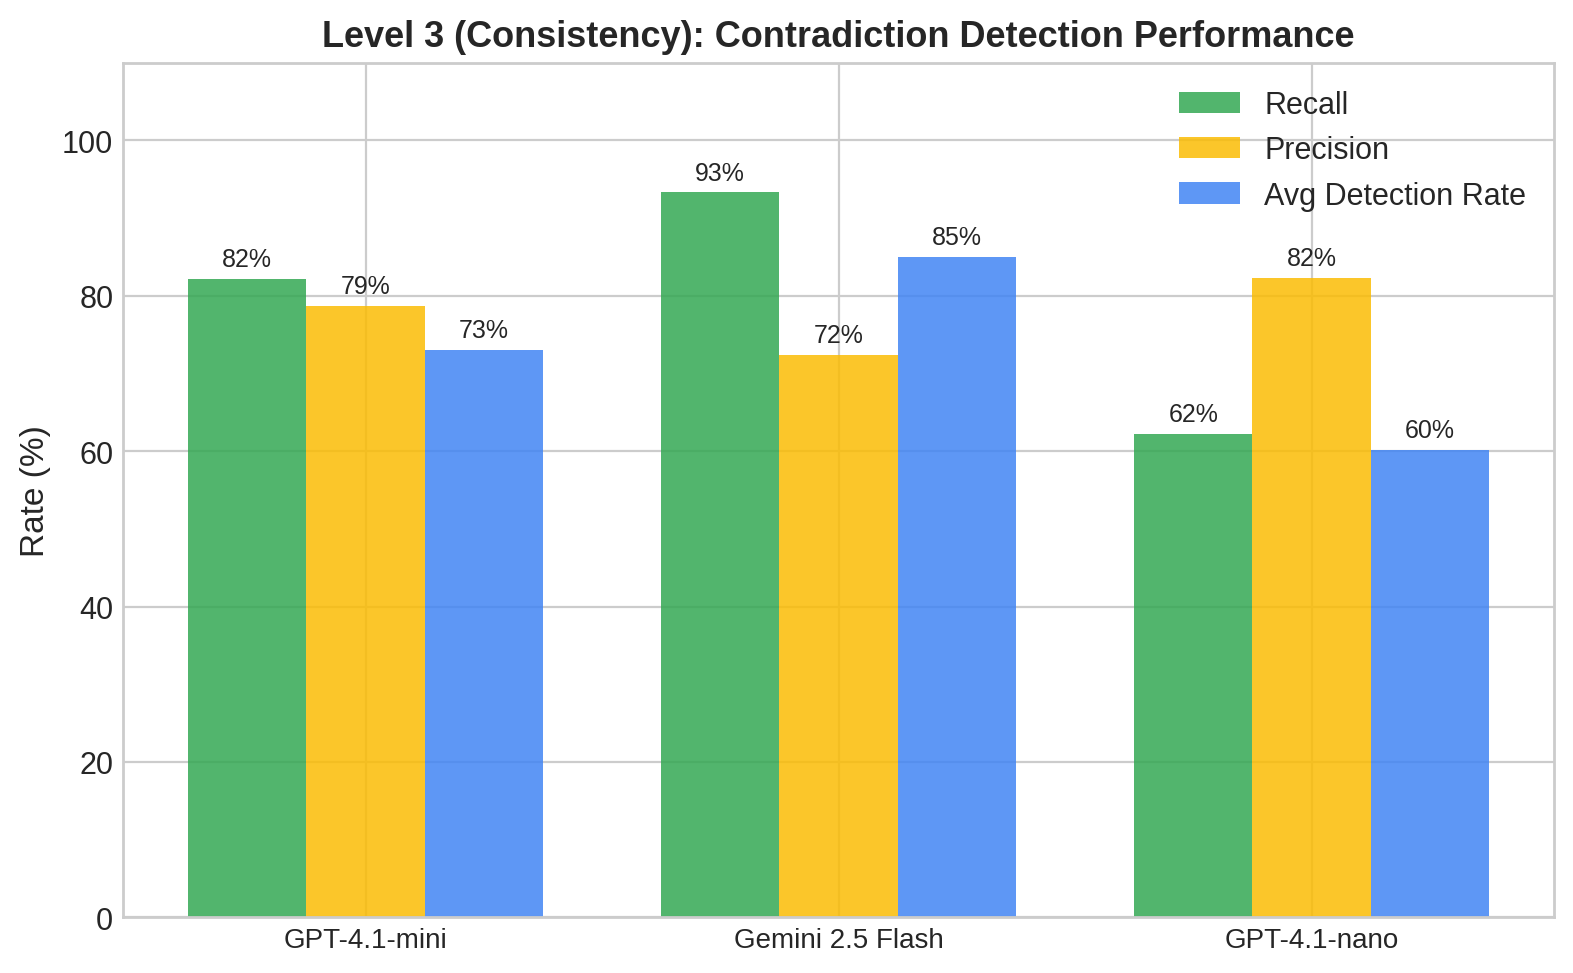
\includegraphics[width=0.8\textwidth]{figures/fig4_consistency.png}
    \caption{Level 3 Consistency Validation. Performance scales with model capability.}
    \label{fig:consistency}
\end{figure}

%% ============================================================================
\section{Analysis and Discussion}
%% ============================================================================

\subsection{Cross-Level Comparison}

\Cref{fig:cross_level} presents a unified view across all three levels. The results reveal a striking pattern: model reliability varies dramatically depending on the \textit{type} of validation required.

\begin{figure}[h]
    \centering
    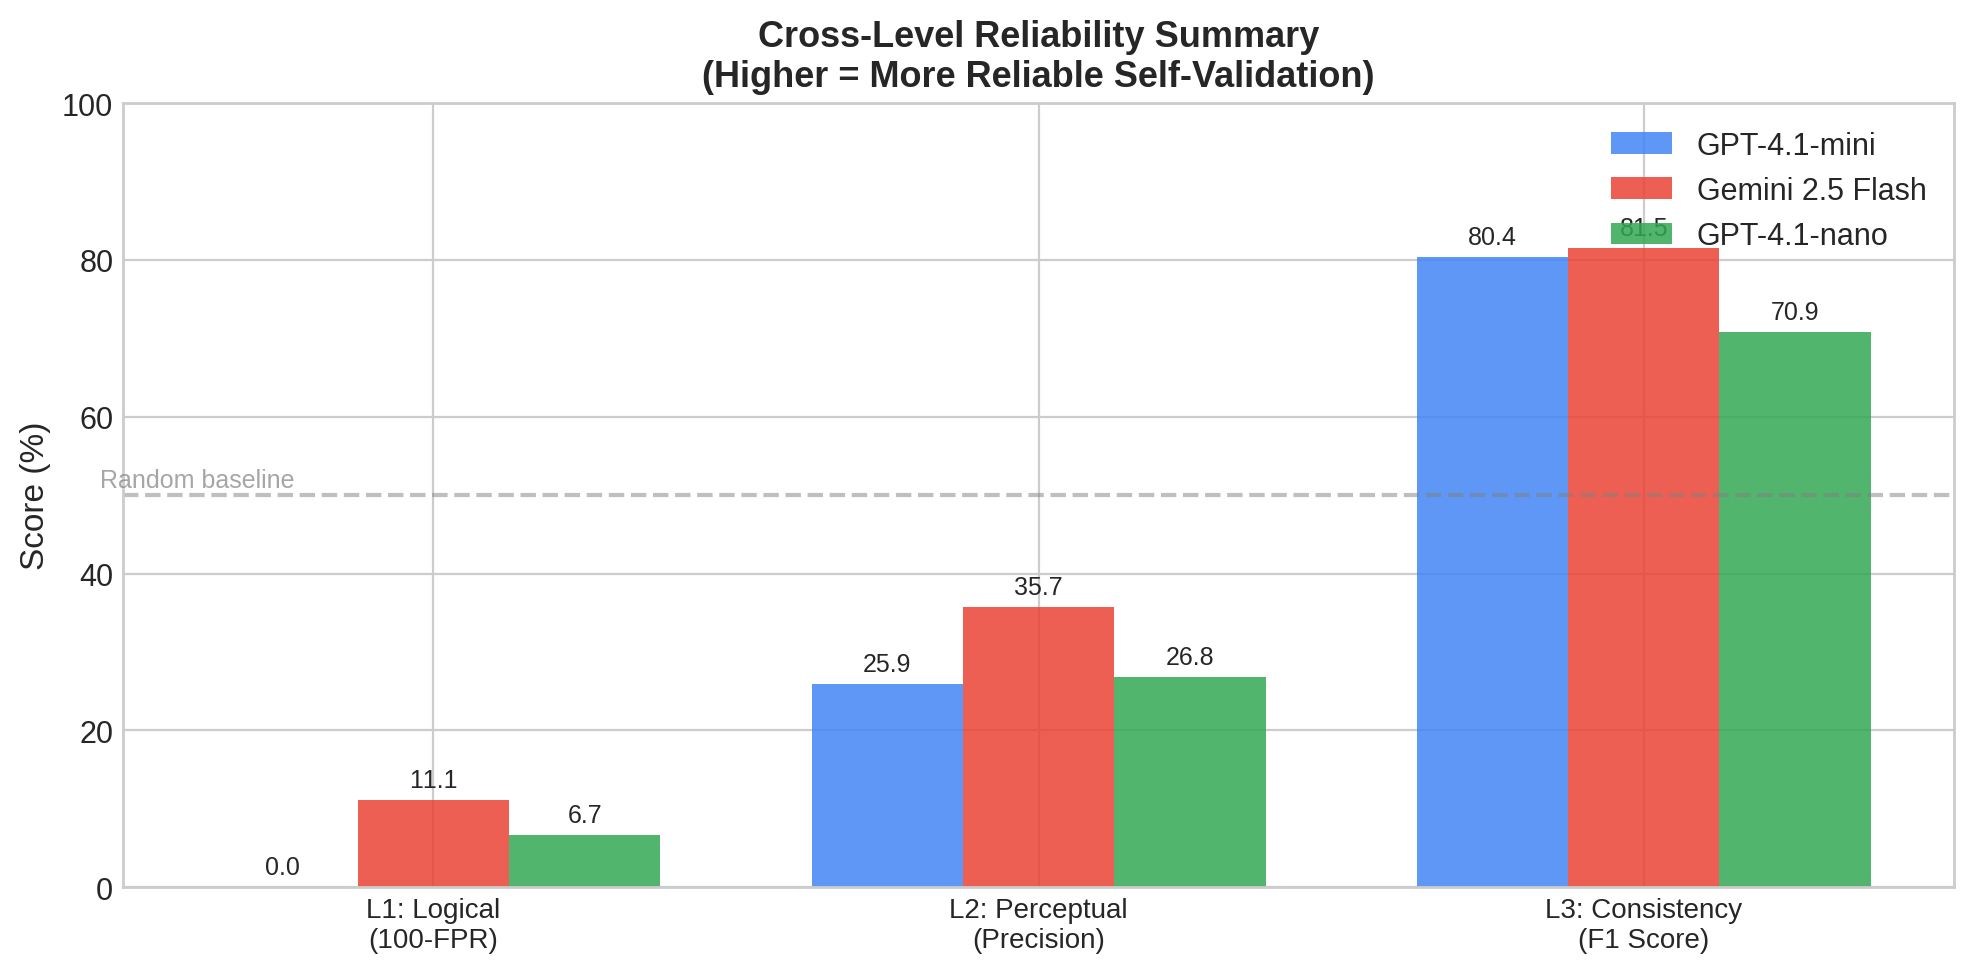
\includegraphics[width=0.85\textwidth]{figures/fig5_cross_level.png}
    \caption{Cross-level reliability comparison across all three validation levels. Higher scores indicate more reliable self-validation.}
    \label{fig:cross_level}
\end{figure}

\textbf{Level 1 (Logical):} Models are maximally unreliable as self-judges. The 66--100\% FPR means that when an agent says ``my code is correct,'' this claim carries almost no information. This is the most dangerous failure mode for autonomous deployment, as it means agents will confidently deliver broken solutions.

\textbf{Level 2 (Perceptual):} Models exhibit the opposite failure mode---they are \textit{too critical} rather than too lenient. While they can detect real bugs, they hallucinate many non-existent ones. This makes them unsuitable as standalone quality checkers but potentially useful as high-recall bug detectors when paired with a human or automated filter.

\textbf{Level 3 (Consistency):} Models are most reliable here, likely because consistency checking operates entirely within their strongest modality (text processing) and requires pattern matching rather than grounded perception or execution-level reasoning.

\subsection{Why Do Models Fail Differently at Each Level?}

We hypothesize three distinct failure mechanisms:

\textbf{Level 1 --- Sycophantic Self-Approval.} When asked to review their own code, models exhibit a strong prior that their output is correct. This is consistent with the sycophancy literature and may be reinforced by RLHF training that rewards confident, affirmative responses.

\textbf{Level 2 --- Ungrounded Knowledge Application.} Models possess extensive knowledge about UI/UX best practices (from training data including web development tutorials, accessibility guidelines, etc.) but cannot \textit{see} the rendered output. They apply rules without verifying whether violations actually manifest, leading to false alarms.

\textbf{Level 3 --- Native Modality Advantage.} Cross-referencing text for contradictions is fundamentally a text-processing task, which aligns with the core competency of LLMs. The high performance here suggests that self-validation failures at other levels are not due to a general inability to be critical, but rather to modality-specific limitations.

\subsection{Implications for Agent Design}

Our findings have direct implications for the design of reliable AI agents:

\textbf{Do not trust self-reported test results.} The extreme ``Yes Man'' bias at Level~1 means that an agent's claim of ``all tests pass'' should be verified by an independent execution environment, not taken at face value.

\textbf{Use LLMs as high-recall bug detectors, not precision tools.} At Level~2, the 100\% recall suggests that LLMs can be effective as a first-pass screening tool for UI bugs, provided their output is filtered by a more precise mechanism (e.g., visual regression testing or human review).

\textbf{Leverage cross-referencing for document quality.} The strong Level~3 performance suggests that LLMs can be effectively deployed for consistency checking in multi-part documents, reports, and codebases.

\subsection{Limitations}

Our study has several limitations. First, the pilot evaluation uses a relatively small sample (10--15 tasks per condition), and results should be validated at larger scale. Second, we evaluate three models (GPT-4.1-mini, Gemini 2.5 Flash, GPT-4.1-nano); future work should expand coverage to Claude 3.5 Sonnet, GPT-4o, Llama 3, and other frontier models. The benchmark is designed to support evaluation of any model via the released harness. Third, the perceptual validation currently uses only HTML source code as input; future work should incorporate rendered screenshots for multimodal evaluation. Fourth, the planted bug paradigm, while scalable, may not capture the full distribution of naturally occurring defects.

%% ============================================================================
\section{Conclusion}
%% ============================================================================

We introduced E$^2$-Bench, the first benchmark to systematically evaluate LLM self-validation reliability across three cognitive levels: logical, perceptual, and consistency validation. Our evaluation of frontier models reveals that current LLMs are unreliable judges of their own work, exhibiting a severe ``Yes Man'' bias in logical validation, an over-reporting tendency in perceptual validation, and moderate reliability in consistency checking. These findings underscore a critical gap: \textbf{the ability to generate is not the ability to evaluate}. As AI agents are deployed in increasingly high-stakes settings, developing robust self-validation mechanisms---and benchmarks to measure them---is essential for safe and reliable autonomy.

\bibliographystyle{plainnat}
\bibliography{references}

\end{document}
